%!TEX root = ../Main.tex
In this section a range of tests will be conducted on different NPG structures in order to uncover the effect of chemical modification of the bridges between the Graphene Nano Ribbons (GNR's) in the NPG. From an applied perspective, one of the main motivations is to find out how these bridges can be chemically modified in order to control the current through the material. A recent study\cite{unpub}, submitted for publication in JACS\footnote{\href{https://pubs.acs.org/journal/jacsat}{Journal of American Chemical Society}}, has shown how one could possibly confine current flow to a single GNR channel by modification of bridges between GNR's in NPG utilising \textit{Quantum Interference} (QI) effects (See \cref{studyfig3}). This provides a solution to an important requirement in carbon-based nanocircuitry design, namely nano confinement of electron flow. The study was focused on the difference in effect of having \textit{meta} and \textit{para} bridges between GNR's. Meta and para bridges are essentially benzene rings connected in two different ways (See \cref{Metaparastructfig}). The meta and para bridges are 'static' cases in the sense that once made through organic synthesis, they are not interchangeable. However, if the bridges are functionalised with oxygen they become sensitive to f.ex. hydrogenation in basic/acidic environments, which tends to affect QI. Thus by hydrogenation it will be possible to tune the electrical properties of the material and make it sensitive to external environments. Studies\cite{li_single_2019} show that hydrogenation of specific sites on nano meter scale is possible experimentally. By the use of the functions developed in previous sections, this section will try to uncover what happens when oxygen is added to the benzene rings in the meta and para bridges. Subsequently hydrogenation of the oxygen will be tested. Following is a section introducing para and meta NPG in detail.
\begin{figure}[h]
		\centering
		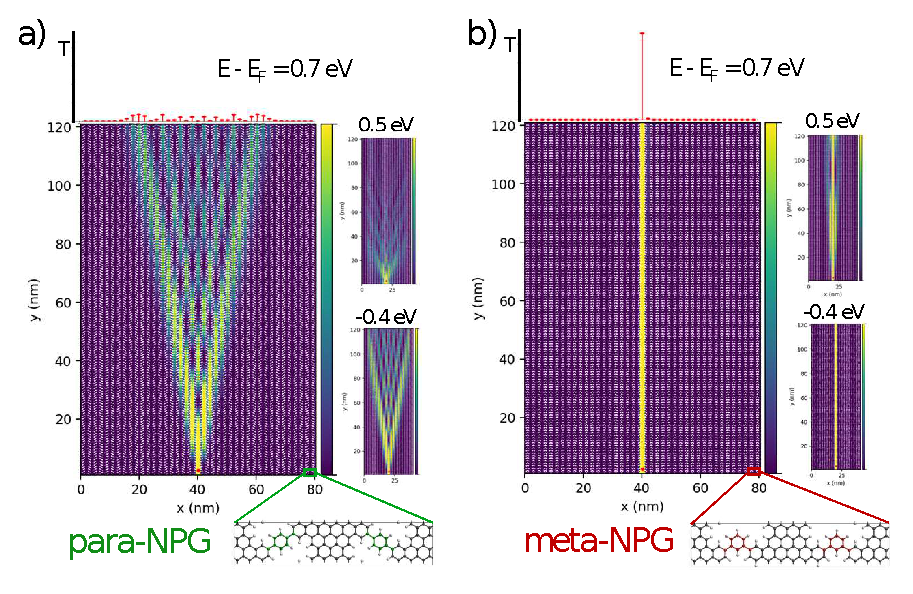
\includegraphics[width = 0.7\textwidth]{Figures/Fig_3.eps}
		\caption{Figure showing the currents through the GNR's in a large peace of NPG. Note how the current is spread across GNR's with the para bridge (a) and confined to a single GNR with meta bridge (b). \textbf{Used with permission of ISAAC}}
		\label{studyfig3}
	\end{figure}
\subsection{Differences in para and meta bridges}\label{metaparasection}
In broad terms the difference in the \textit{meta} and \textit{para} structures lies in the path an electron will travel through the benzene ring to get across the bridge between GNR's in NPG. In the para bridge, the path across the aromatic ring is symmetric and so the electron will pass above or below with equal probability. Since the para bridge has three bonds in each direction across the ring, the path length in the para bridge is the same on each side (See \cref{Metaparastructfig} a)). This will cause constructive QI of the states once the waves meet on the other side of the ring. Which for para NPG causes electronic coupling between the GNR channels. For the meta bridge the way across the aromatic ring is not symmetric in the sense that there is two bonds across the path below and four bonds across on the path above (See \cref{Metaparastructfig} b)). This will cause a shift by half a wavelength between the two paths and thus create destructive QI between waves meeting on the other side of the ring. In the meta NPG, this causes electronic decoupling between GNR channels, allowing for confinement of injected currents in a single GNR channel\cite{unpub}. In \cref{metapara} band plots as well as transmission plots are shown for para and meta NPG. In the band plots the two sets of valence/conduction bands around the fermi level shows a shift for para and interference for meta NPG. Looking at the transmission plots directly below one can see there is transmission  and thus coupling of the states between the GNR's for para. The area between the two peaks at \SI{0.5}{\electronvolt} and  \SI{1.2}{\electronvolt} show transport between the GNR's. In the transmission plot for meta the transmission is confined. In the transmission plot the area between the two peaks is now pretty much 0. This means that  states occurs between GNR's are decoupled in meta system. To summarise these results qualitatively: Shifts of the bands in the band plots, corresponds to effective coupling of the states between the GNR's. Bands on top of each other, showing QI, corresponds decoupling of the states to a single GNR thus decoupling states between GNR's. In the following sections, band plots will mainly be used to show results. Therefore one should keep in mind how the band structures, qualitatively, relate to transmission. In \cref{appfigs}, \cref{allbands} a figure obtained from the developed functions with band plots of normal, para and meta NPG can be seen.
\begin{figure}[ht]
    \centering
    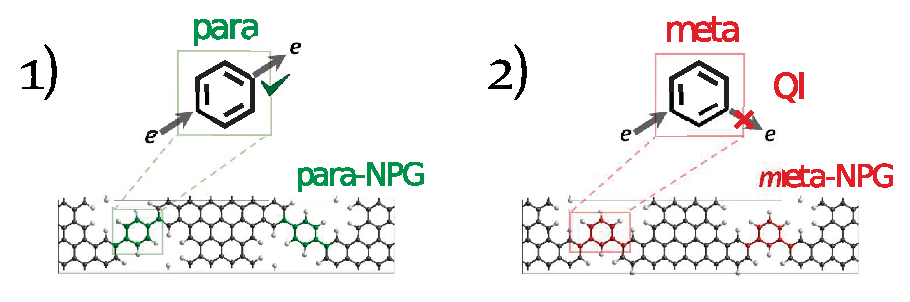
\includegraphics[width=0.8\textwidth]{Figures/Metaparagraphic.eps}
    \caption{a) showing the para NPG, b) showing the meta NPG. Used with permission from \textbf{Isaac}}
    \label{Metaparastructfig}
\end{figure}
\begin{figure}[ht]
	\centering
	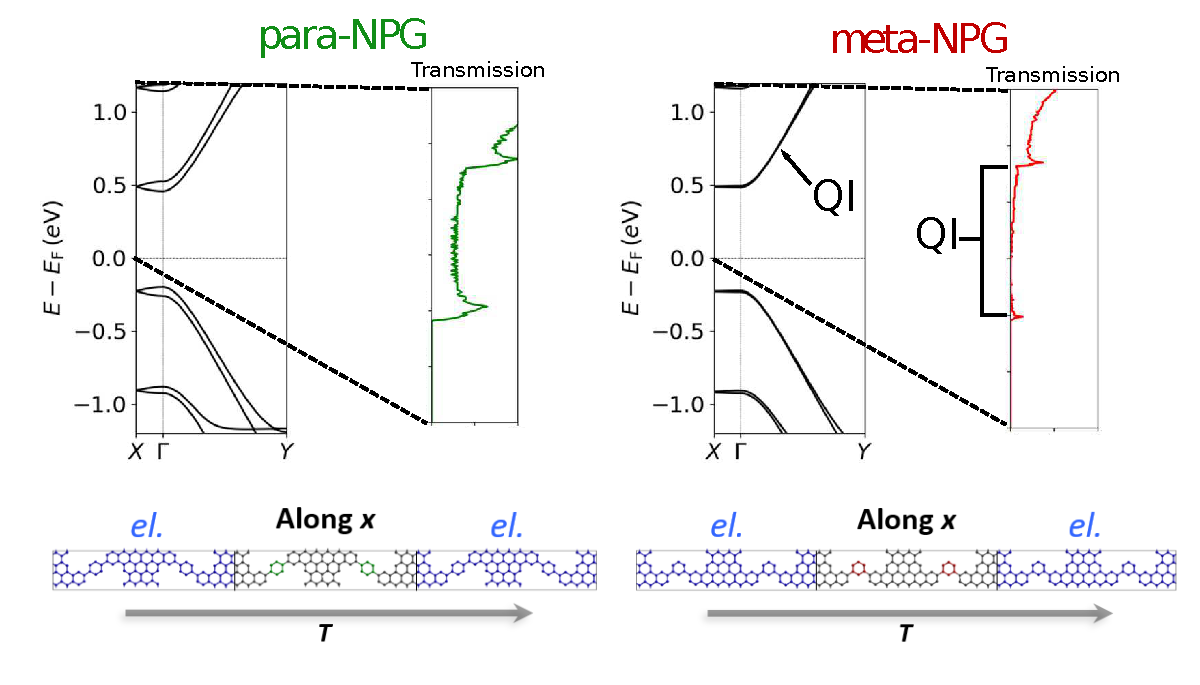
\includegraphics[width=0.8\textwidth]{Figures/metapararesultdraft.eps}}
	\caption{Figure showing band plots and transmission plots for para and meta NPG. In the bottom of each plot is a schematic showing which way the transmission occurs in relation to the NPG.\textbf{Used with permission of ISAAC}}
	\label{metapara}
\end{figure}
\newpage
\subsection{Tests with modified meta and para NPG}\label{test1}
The tests consist of two kinds of chemical modification. Firstly it will be adding oxygen sites to the meta and para NPG (Addition of Oxygen will be simulated by addition of another carbon site to the structure, effectively adding another pi-electron). Secondly simulations of hydrogenation will be done by having added hydroxide groups. By removing hydroxide sites entirely, the aim is to simulate the removal of the extra pi-electron which the oxygen originally provided, but now lost by hydrogenation. These modifications will be carried out separately. The band plots obtained via DFT makes it hard to understand what is actually going on in the system chemically. Therefore the aim is to show that using the methods developed, based on Tight Binding models, it is possible to reproduce bands structures calculated from DFT. If successful, it will provide a much easier way to understand the effect of the implemented chemical modification compared to the DFT approach. Band plots, as well as some on-site potential maps, calculated with DFT has been provided by \textit{Isaac} for comparison. The geometries, on which the calculations are used, are optimised by DFT. They will also be provided by \textit{ISAAC}.
\subsection{Test 1: Para-O\mathinhead{_4}{_4}-NPG}
In the first test is considering the Para-O\(_4\)-NPG. The basis structure is para-NPG where 4 oxygen sites are bonded, two on each benzene ring (See \cref{PS4OOW} ). The fist thing to notice is that in \cref{PS4ODFT} the valence band show QI and thus decouples the GNR's. So in spite having a para bridge, decoupling occurs when oxygen in bonded to the ring. To simulate this practically, the developed method considers the bonded oxygen as carbon atoms. It does not differentiate between the type of atoms only the distance between them. As a baseline the potential of these atoms are thus the same. Moreover, the hydrogen, included in the provided optimised geometries, will be removed before any calculations take place. In \cref{PS4Odevnomod} one can see the resulting band structure plot, where calculations have been carried out, using only the provided geometry. No modifications where made. The band plot does not show much resemblance with the one obtained, using DFT. It is pretty much symmetric around the fermi level and it is hard to make out whether there is coupling or decoupling between GNR's. This is expected. As seen in the potential map of \cref{potmapPS4O}, the sites where the oxygen is bonded, have a potential much different from that of the rest of the system (the four dark blue spots). As mentioned, the baseline of the method does not take into account differentiating on-site potentials within a cell. So to compensate for this, the on-site potential of the four bonded oxygen is changed. In \cref{PS4Odevmod} one can see the resulting band plot after the on-site potential of the bonded oxygen has been change to \SI{-0.50}{\electronvolt}. The resulting band plot resembles the DFT calculations much more. There is now QI in the valence bands which means decopling of the GNR's.
\begin{figure}[ht]
	\centering
	\begin{subfigure}[b]{0.8\textwidth}
		\centering
		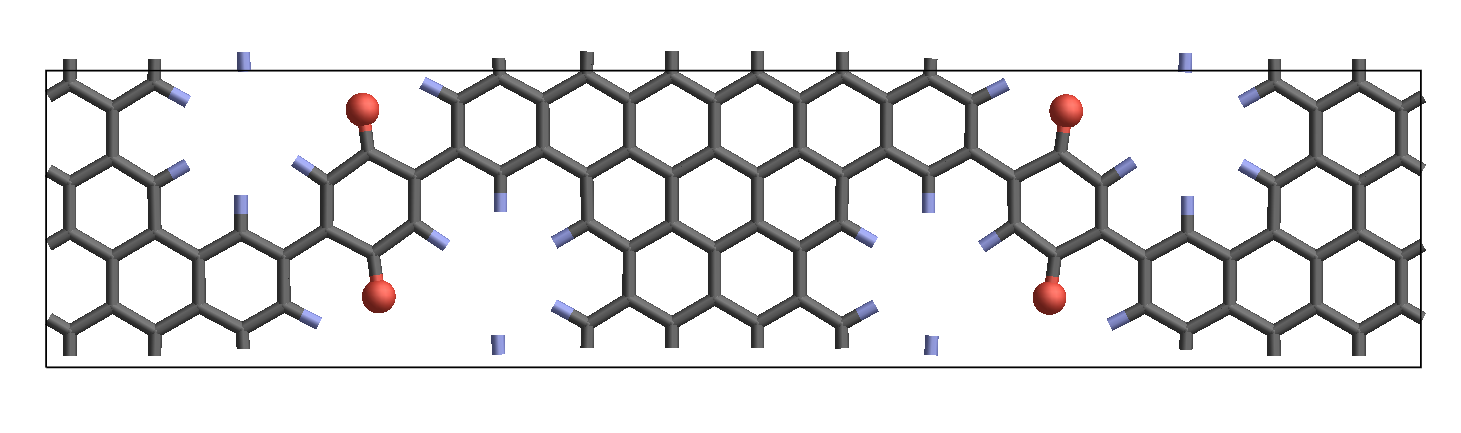
\includegraphics[width=0.8\textwidth]{Figures/para_O4.png}
		\vspace{-1\baselineskip}
		\caption{}
		\label{PS4OOW}
	\end{subfigure}
	\vskip
	\begin{subfigure}[b]{0.3\textwidth}
		\centering
		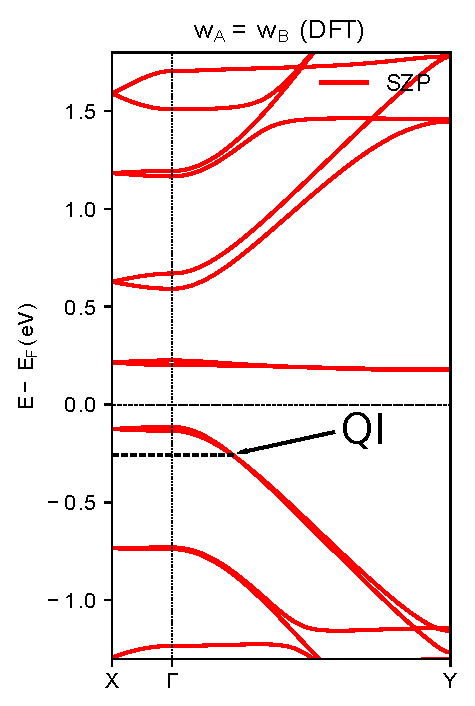
\includegraphics[width=0.8\textwidth]{Figures/PS4ODFT.eps}
		\vspace{-1\baselineskip}
		\caption{}
		\label{PS4ODFT}
	\end{subfigure}
	\hspace{-30pt}
	\begin{subfigure}[b]{0.3\textwidth}
		\centering
		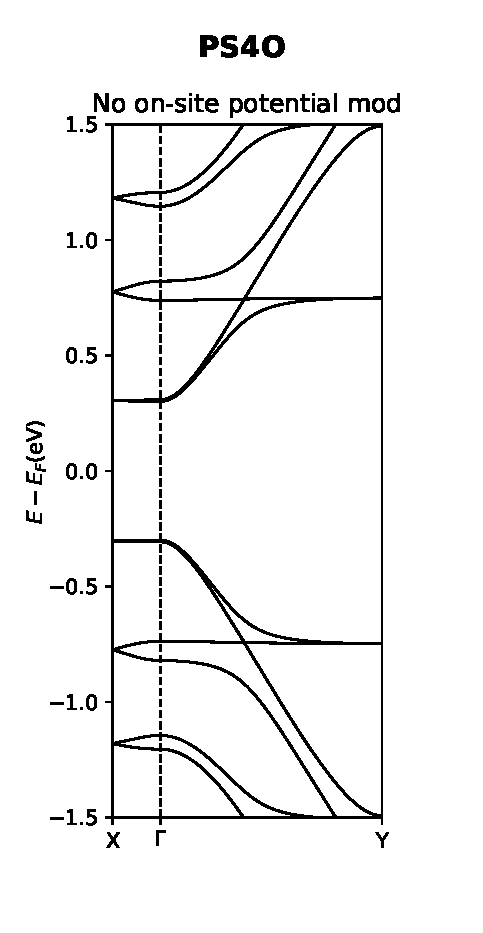
\includegraphics[width=0.8\textwidth]{Figures/PS4Onomod.eps}
		\vspace{-2\baselineskip}
		\caption{}
		\label{PS4Odevnomod}
	\end{subfigure}
	\begin{subfigure}[b]{0.3\textwidth}
		\centering
		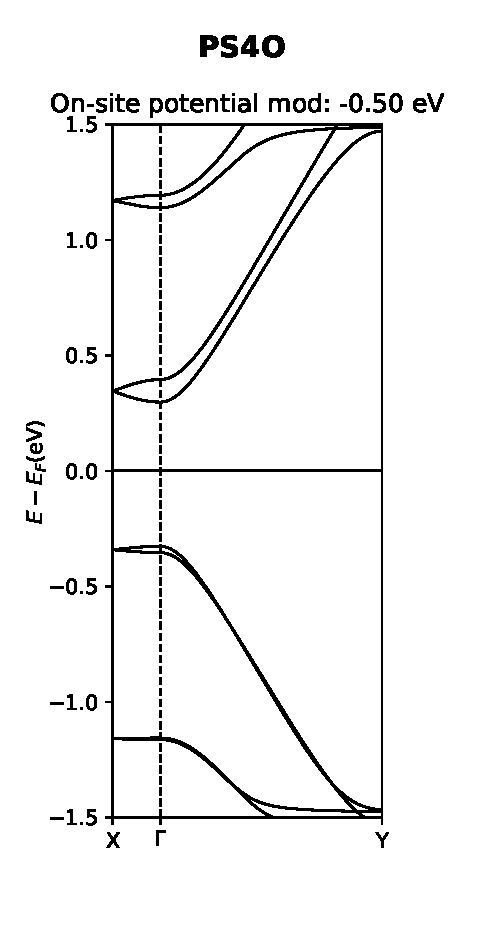
\includegraphics[width=0.8\textwidth]{Figures/PS4Omod.eps}
		\vspace{-2\baselineskip}
		\caption{}
		\label{PS4Odevmod}
	\end{subfigure}
	\vskip
	\begin{subfigure}[b]{0.8\textwidth}
		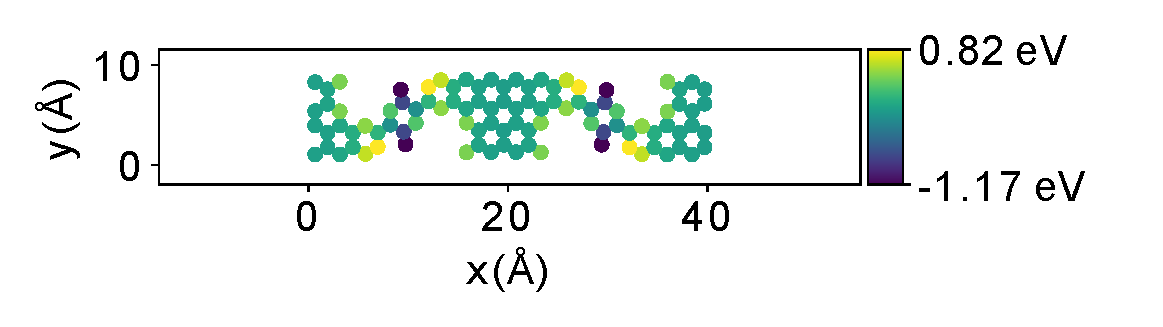
\includegraphics[width=0.8\textwidth]{Figures/PS4O.eps}
		\vspace{-1\baselineskip}
		\caption{}
		\label{potmapPS4O}
	\end{subfigure}
	\caption{Figure showing the band structure obtained using DFT a), band structures obtained using developed program with no on-site potential mods b) and with the on-site potential changed to \SI{-0.5}{\electronvolt} c). Lastly a potential map of the system d)}
	\label{PS4O}
\end{figure}
\subsection{Test 2: P-(OH)\mathinhead{_4}{_4}-NPG}\label{test2}
Next test will be with the P-(OH)\(_4\)-NPG system. Again the basis structure is para-NPG with added oxygen, but here the aim is to simulate hydrogenation, so therefore the oxygen atoms added will become hydroxide groups (See \cref{PS4OHOW}). The DFT plot in \cref{PS4OHDFT} shows a shift in the valence/conduction bands, so the GNR's have been coupled again. Here the approach is to try use the applied on-site potential for the bonded oxygen from the previous test. This After removal the caluculations are done as usual. The resulting plot in \cref{PS4OHremove} Here the test is to show the difference between removing a OH site entirely (effectively the hydrogen in hydroxide removes the extra pi-electron in oxygen from the system, which can be simulated by removing the atoms entirely) and lowering the on-site potential of the oxygen in the OH group significantly in relation to the rest of the system. Again the results from DTF is shown in \cref{PS4OHDFT} and following the band plots from the developed scripts (\cref{PS4OHremove,PS4OHmod1,PS4OHdevmod2}).
\begin{figure}[ht]
	\centering
		\begin{subfigure}[b]{0.8\textwidth}
		\centering
		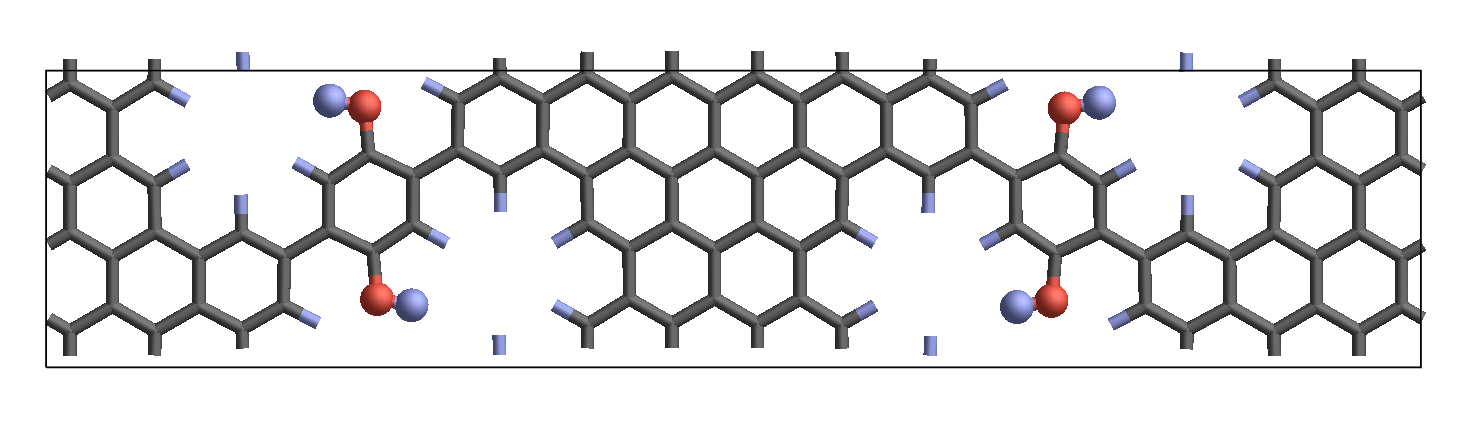
\includegraphics[width=0.8\textwidth]{Figures/para_OH4.png}
		\vspace{-1\baselineskip}
		\caption{}
		\label{PS4OHOW}
	\end{subfigure}
	\vskip
	\begin{subfigure}[b]{0.3\textwidth}
		\centering
		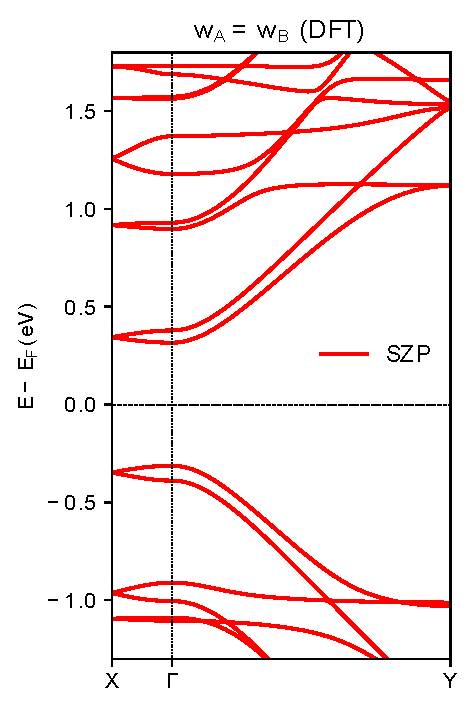
\includegraphics[width=0.8\textwidth]{Figures/PS4OHDFT.eps}
		\vspace{-1\baselineskip}
		\caption{}
		\label{PS4OHDFT}
	\end{subfigure}
	\hspace{-30pt}
	\begin{subfigure}[b]{0.3\textwidth}
		\centering
		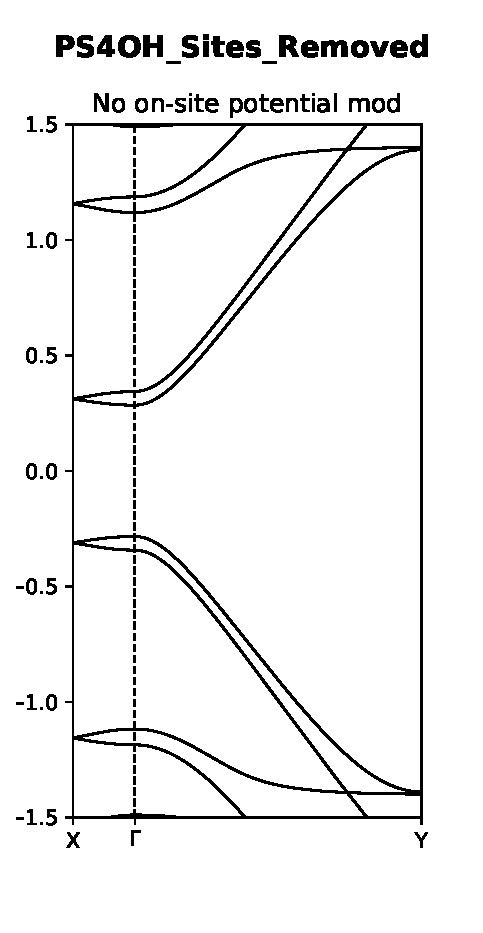
\includegraphics[width=0.8\textwidth]{Figures/PS4OHSitesRemoved.eps}
		\vspace{-2\baselineskip}
		\caption{}
		\label{PS4OHremove}
	\end{subfigure}
	\begin{subfigure}[b]{0.3\textwidth}
		\centering
		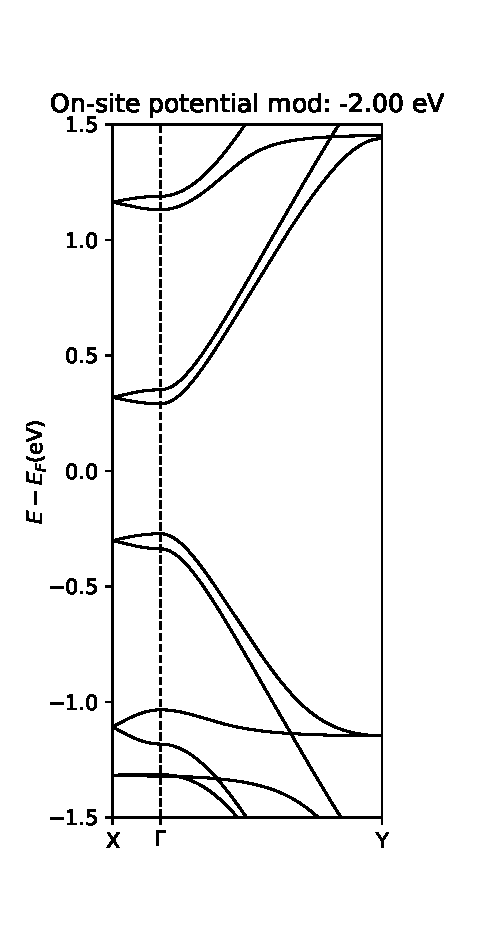
\includegraphics[width=0.8\textwidth]{Figures/PS4OHmod.eps}
		\vspace{-2\baselineskip}
		\caption{}
		\label{PS4OHdevmod2}
	\end{subfigure}
	\vskip
	\begin{subfigure}[b]{0.8\textwidth}
		\centering
		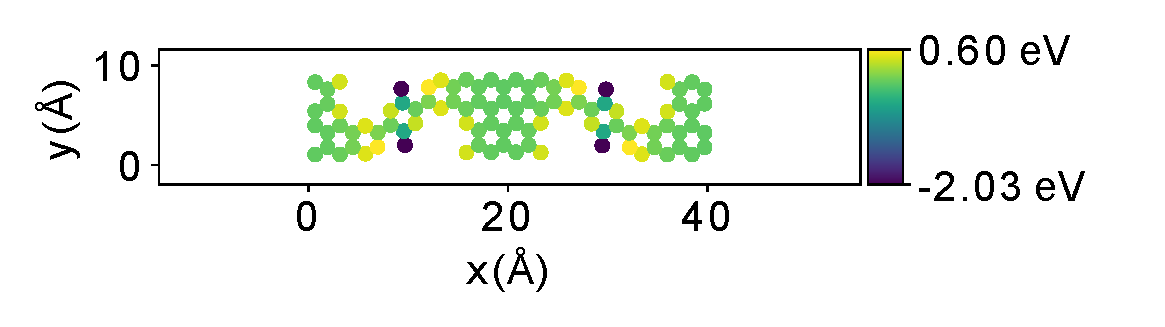
\includegraphics[width=0.8\textwidth]{Figures/PS4OH.eps}
		\vspace{-1\baselineskip}
		\caption{}
		\label{potmapPS4OH}
	\end{subfigure}
	\caption{Figure showing the band structures obtained using DFT a), band plot where the added sites have been removed b), a potential map of the system c), band plot where the on-site potential has been changed by \SI{-2.5}{\electronvolt} d), and band plot where the on-site potential has been changed by \SI{-2.0}{\electronvolt} e).}
	\label{PS4OH}
\end{figure}
Multiple on-site potentials as well as removal of the specific atomic sites were tested to see which one came closest to that of the band structures in \cref{PS4OHDFT}. The removal was done by removing specific coordinates in the given files before it was run through the script. A seen in \cref{PS4OHremove} the effect of removing the sites gives a plot, somewhat in agreement with \cref{PS4OHDFT}. However the lowest and highest bands does not show. The two other plots in \cref{PS4OHmod1,PS4OHdevmod2} show how gradually changing the on-site potential gets better and better agreement with DFT. A on-site potential of \(\SI{-2.5}{\electronvolt}\) proved to be a bit too high, though still showing good agreement. Lowering the potential to \(\SI{-2.0}{\electronvolt}\) which is the value similar to that given by the lowest potential in the potential map \cref{potmapPS4OH}, yielded a result that is pretty much spot on, considering the valence bands, when compared with DFT.
\subsection{Test 3: Meta-NPG with oxygen added symmetrically}\label{test3}
This test is done in the same manner as \cref{test1}. The only difference being that the system is different. Here the basic system is the meta-NPG and two oxygen have been added symmetrically with respect to the periodically repeating GNR's (See \cref{appfigs}, \cref{Strucow}, no. 1). As seen in \cref{MS2O} three band plots have been produced to compare with the fourth which is from DFT calculations. In general it spreading of the bands is observed even though the basic structure is meta. Meta should according to the results mentioned in \cref{metaparasection} confine the transmission but this is not what is seen in these results. The explanation is that the added oxygen provides an extra pi-electron to the system, thus allowing for some transmission between GNR's.
\begin{figure}[ht]
	\centering
		\begin{subfigure}[b]{0.8\textwidth}
		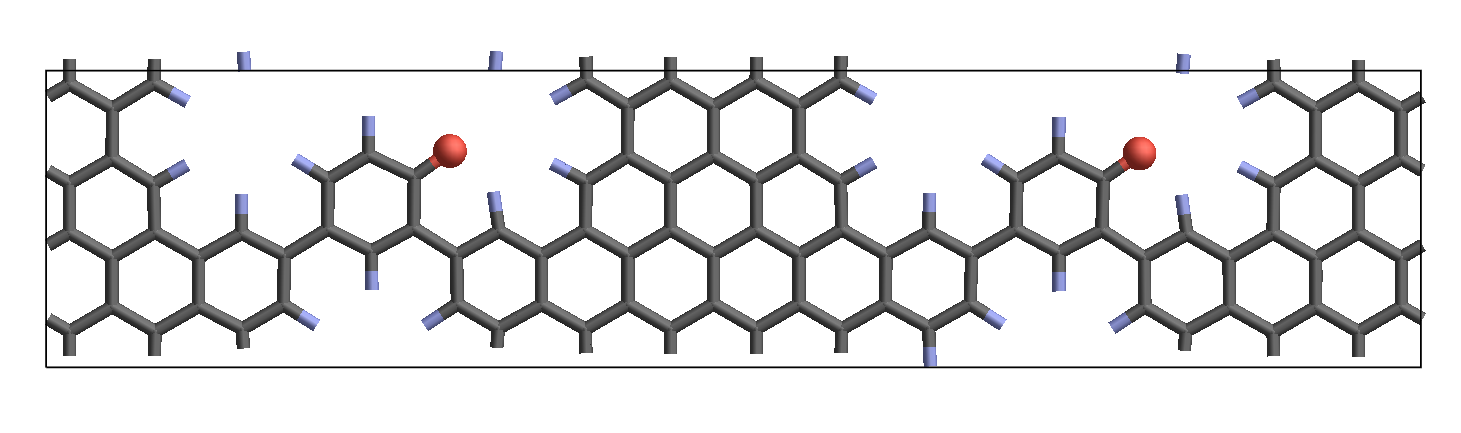
\includegraphics[width=0.8\textwidth]{Figures/meta_O4.png}}
		\vspace{-1\baselineskip}
		\caption{}
		\label{MS2OOW}
	\end{subfigure}
	\vskip
	\begin{subfigure}[b]{0.3\textwidth}
		\centering
		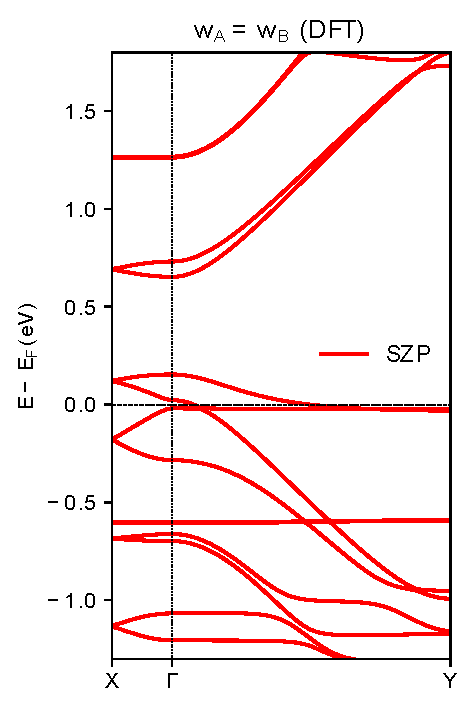
\includegraphics[width=0.8\textwidth]{Figures/MS2ODFT.eps}
		\vspace{-1\baselineskip}
		\caption{}
		\label{MS2ODFT}
	\end{subfigure}
	\hspace{-30pt}
	\begin{subfigure}[b]{0.3\textwidth}
		\centering
		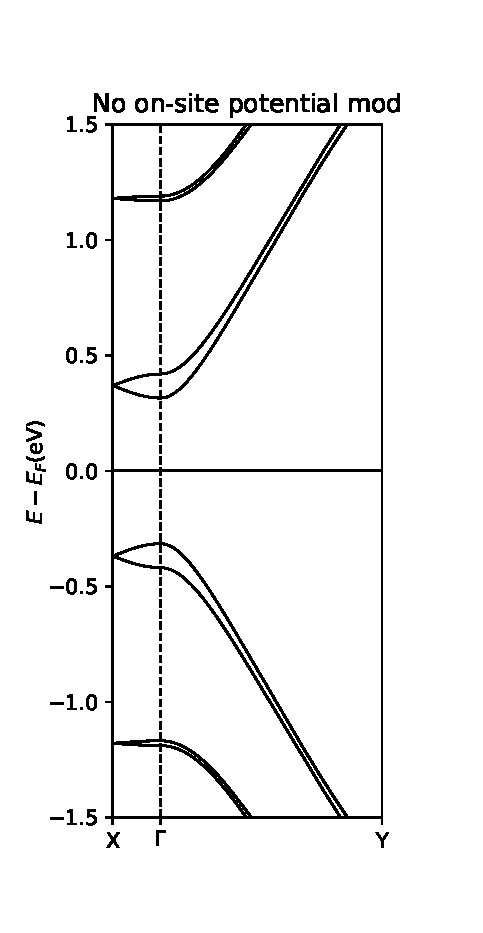
\includegraphics[width=0.8\textwidth]{Figures/MS2Onomod.eps}
		\vspace{-2\baselineskip}
		\caption{}
		\label{MS2Odevnomod}
	\end{subfigure}
	\begin{subfigure}[b]{0.3\textwidth}
		\centering
		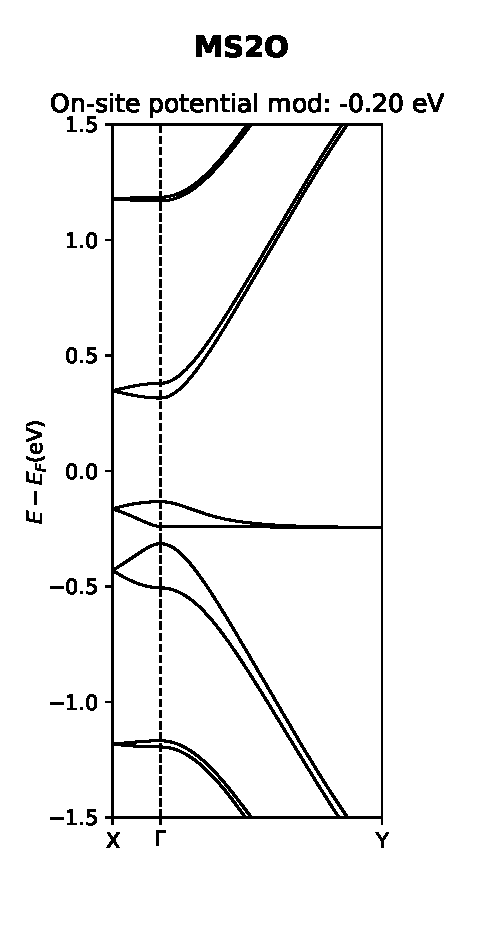
\includegraphics[width=0.8\textwidth]{Figures/MS2Omod.eps}
		\vspace{-2\baselineskip}
		\caption{}
		\label{MS2Odevmod}
	\end{subfigure}
	\vskip
	\hspace{4pt}
	\begin{subfigure}[b]{0.8\textwidth}
		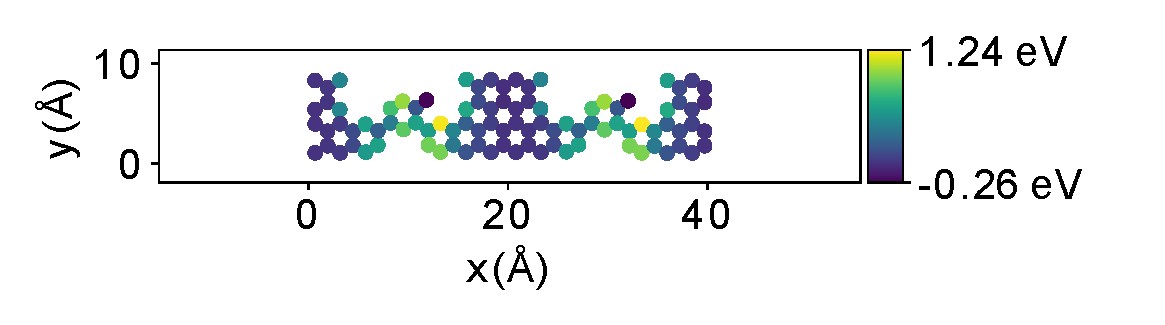
\includegraphics[width=0.8\textwidth]{Figures/MS2Opotmap.eps}
		\vspace{-1\baselineskip}
		\caption{}
		\label{potmapM2SO}
	\end{subfigure}
	\caption{Figure showing the band structure obtained using DFT a), band structures obtained using developed program with no on-site potential mods b) and with the on-site potential changed to \SI{-0.2}{\electronvolt} c). Lastly a potential map of the system d)}
	\label{MS2O}
\end{figure}
In \cref{MS2Odevnomod} the bands at the fermi level show QI in all directions. This is not in good agreement with the DFT plot. The DFT plot seem to have this straight band located further down around \SI{-0.58}{\electronvolt}. However, is the on-site potential of the oxygen is changed, the match with DFT is much better. In \cref{MS2Odevmod} there is spreading of the bands in the centre like the DFT plot. The spreading of the next set of bands is also larger, showing good agreement with DFT.
\subsection{Test 4: Simulating hydrogenation of meta-NPG with symmetrically added oxygen}\label{test4}
The fourth and final test will be with the same approach as \cref{test2} only here the hydrogenation is of the meta-NPG with oxygen added symmetrically (See \cref{appfigs}, \cref{Strucow}, no. 2). In \cref{MS2OH} the result of the test are shown. Now that the oxygens have hydrogenated the extra pi-electron provided is taken by hydrogen. This means that the system is similar to the regular meta system discussed in \cref{metaparasection}.
\begin{figure}[ht]
	\centering
		\begin{subfigure}[b]{0.8\textwidth}
		\centering
		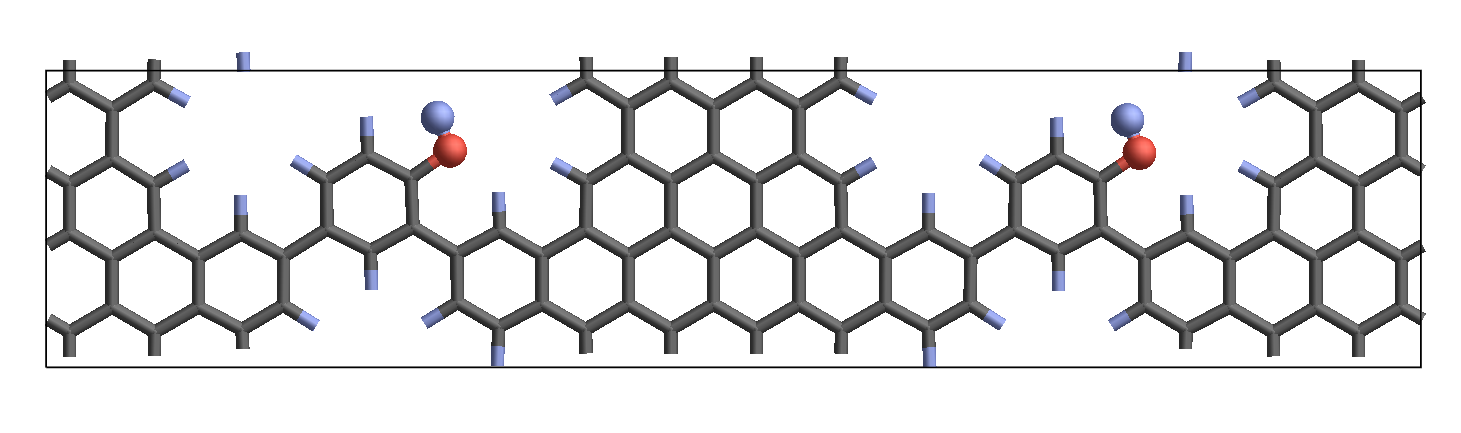
\includegraphics[width=0.8\textwidth]{Figures/meta_OH4.png}}
		\vspace{-1\baselineskip}
		\caption{}
		\label{MS2OHOW}
	\end{subfigure}
	\vskip
	\begin{subfigure}[b]{0.3\textwidth}
		\centering
		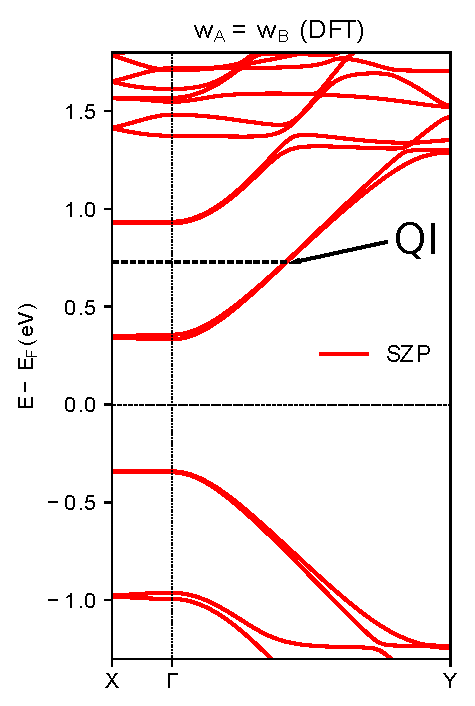
\includegraphics[width=0.8\textwidth]{Figures/MS2OHDFT.eps}
		\vspace{-1\baselineskip}
		\caption{}
		\label{MS2OHDFT}
	\end{subfigure}
	\hspace{-30pt}
	\begin{subfigure}[b]{0.3\textwidth}
		\centering
		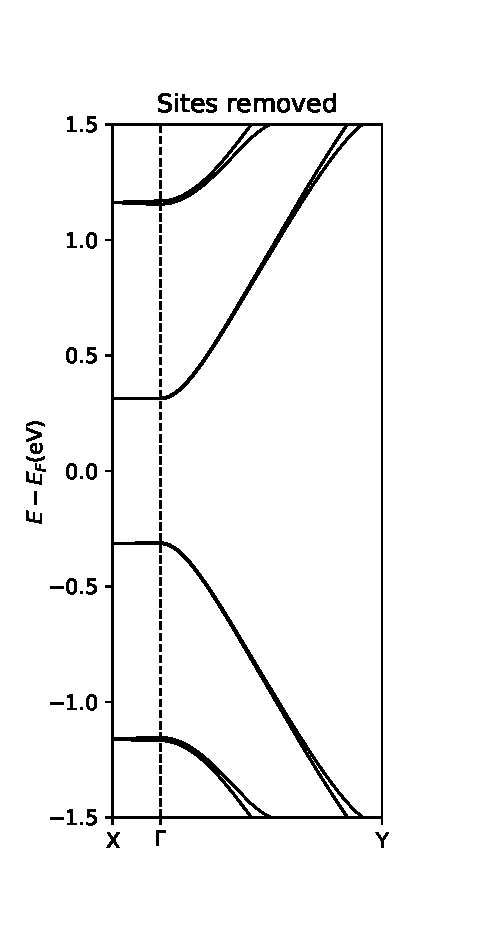
\includegraphics[width=0.8\textwidth]{Figures/MS2OHSitesRemoved.eps}
		\vspace{-2\baselineskip}
		\caption{}
		\label{MS2OHremove}
	\end{subfigure}
	\begin{subfigure}[b]{0.3\textwidth}
		\centering
		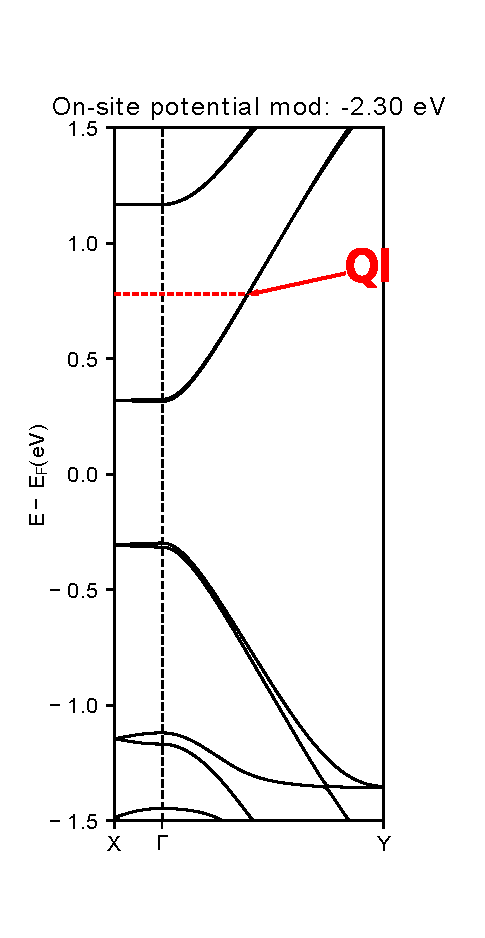
\includegraphics[width=0.8\textwidth]{Figures/MS2OHmod.eps}
		\vspace{-2\baselineskip}
		\caption{}
		\label{MS2OHdevmod2}
	\end{subfigure}
	\vskip
	\hspace{2pt}
	\begin{subfigure}[b]{0.8\textwidth}
		\centering
		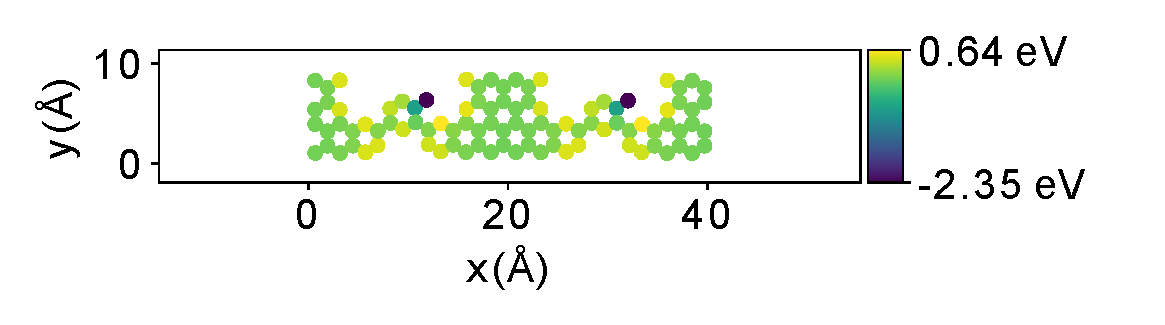
\includegraphics[width=0.8\textwidth]{Figures/MS2OH.eps}
		\vspace{-1\baselineskip}
		\caption{}
		\label{potmapMS2OH}
	\end{subfigure}
	\caption{Figure showing the band structures obtained using DFT a), band plot where the added sites have been removed b), a potential map of the system c), band plot where the on-site potential has been changed by \SI{-1.5}{\electronvolt} d), and band plot where the on-site potential has been changed by \SI{-2.3}{\electronvolt} e).}
	\label{MS2OH}
\end{figure}
One can see QI in all three plots in \cref{MS2OH} obtained from the developed scripts. And the all show relatively good agreement with the DFT plot. However, the best result came from tweaking the on-site potential to \SI{-2.3}{\electronvolt} as seen in \cref{MS2OHdevmod2}. Comparing the plots with the regular meta system from \cref{metaparasection} indeed show good agreement as well.
\subsection{Test summary}
For the para systems, the added oxygen introduced some QI to the system. It was possible to show that the developed program could reproduce the results obtained from DFT. This did require some adjustment to the on-site potential of the added oxygen. By hydrogenation of the oxygen it was shown that the system again returned to spreading of the bands. Again by adjusting the on-site potential it was possible to obtain results very close to the DFT calculation. The results are also comparable with the ones mentioned in \cref{metaparasection}. This shows that hydrogenation of oxygen can change the system to resemble regular para-NPG, even if it has oxygens added. For the meta systems it was shown the it is possible to manipulate the system. First by having some transmission between GNR's by adding in oxygen as in \cref{test3}. Then by hydrogenating the system in\cref{test4}, getting QI and thus confinement. This turned out to be similar to un-modified meta NPG.
All in all these results give a better, intuitive understanding of what happens with the electron transport in NPG. This is because all manipulations can be followed with ease and the results are easy to interpret.
